%------------------------------------------------
% Event.tex
%
% This document build the incident frame
%------------------------------------------------
\section{Event Management}
\frame
{
\frametitle{Contenuti}
\tableofcontents[currentsection]
%\addtocounter{framenumber}{-1}
}

\subsection*{Input e Output}
\begin{frame}{Input e Output}
Input:
\begin{table}
\begin{tabular}{ l | c }
\textbf{Input} & \textbf{Da}\\
\hline
Alimentazione elettrica & UPS\\
Notifiche hardware & hardware\\
Traffico di rete & firewall\\
Traffico su dati & DBMS\\
Log applicativi & Applicazioni\\
Notifiche accessi/uscite & Sistemi controllo accessi\\
Notifiche di emergenza & Sensori\\
\end{tabular}
\caption{input di processo}
\end{table}
Output:
\begin{table}
\begin{tabular}{ c | c }
\textbf{Output} & \textbf{Da}\\
\hline
Ticket & Service Desk\\
\end{tabular}
\caption{output di processo}
\end{table}
\end{frame}

\subsection*{Attività di processo}
\begin{frame}{Attività di processo}
\begin{figure}
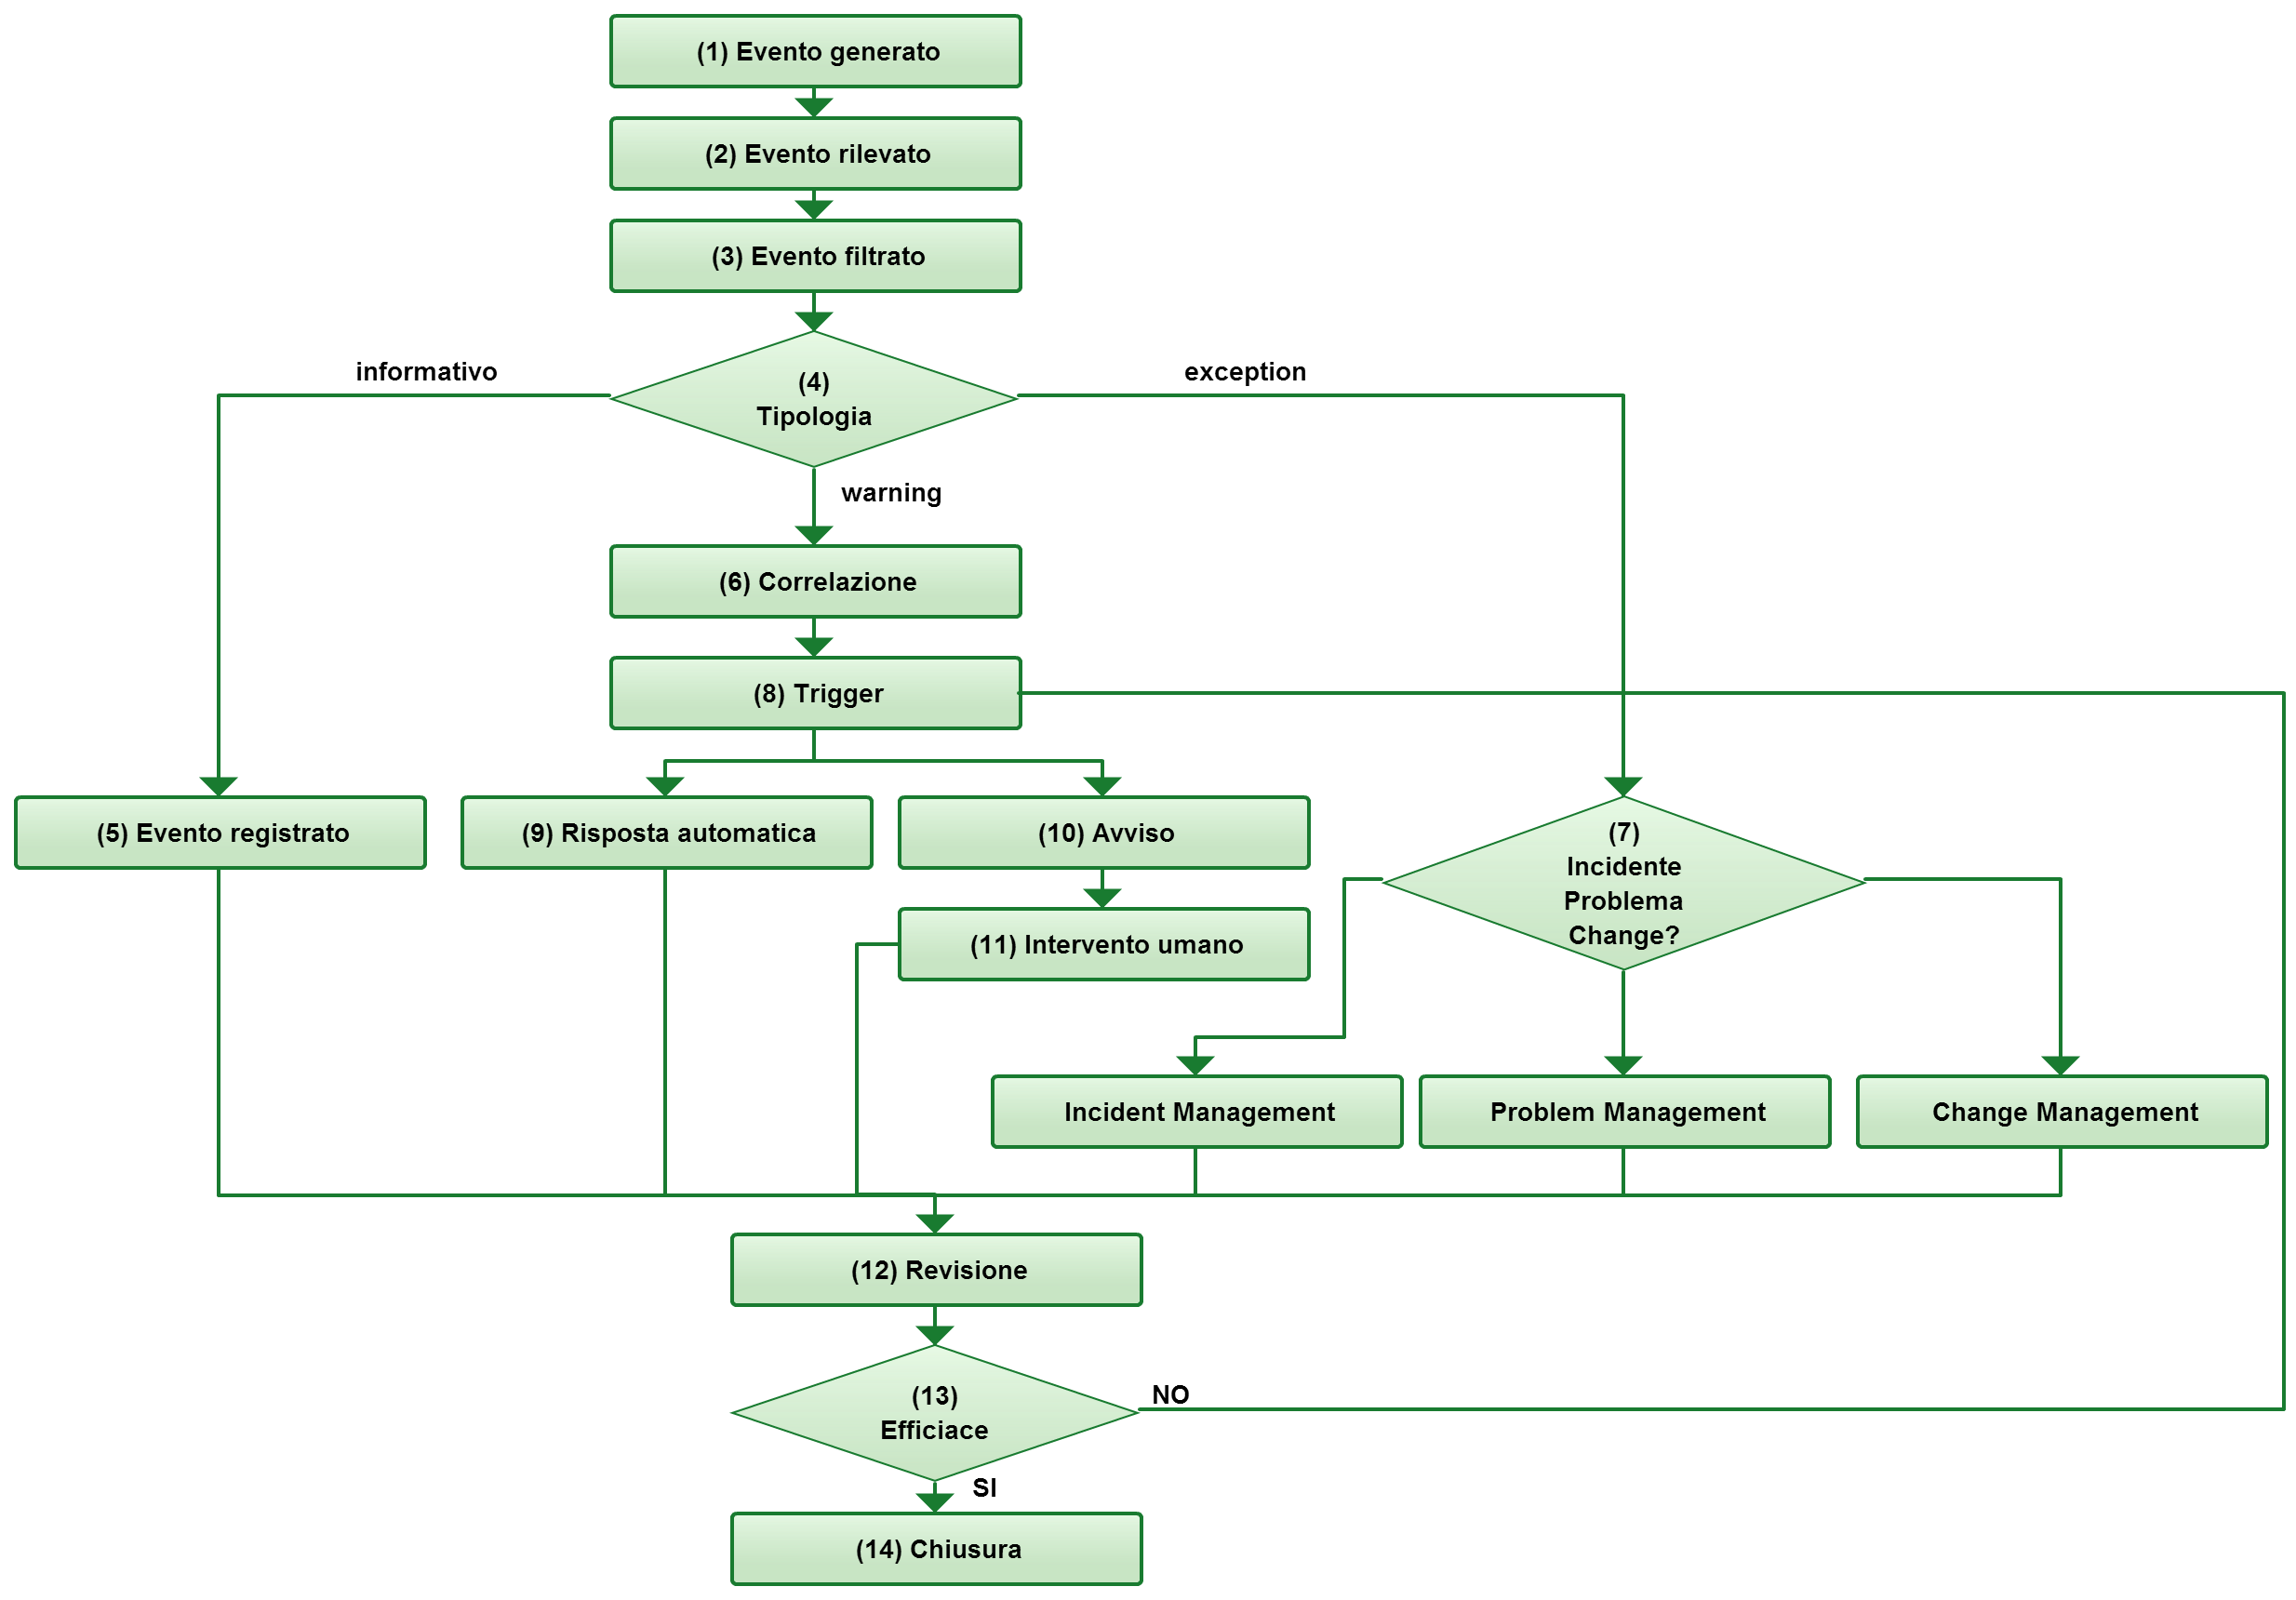
\includegraphics[scale=0.22]{Images/Event_management.png}
\end{figure}
\end{frame}